%1. Introduction

%2. Base technology !!! RENAME
	%WebRTC
	%P2P
	%Authentication
	%Trust model

%3. Shared design (Top level design)
	%Program Flow
	%Specific implementation (of technology)
	%extendability

%4. Specific design
	%Serverless
		%Use Case
		%Program Flow
		%Specific implementation (of technology)

	%Assisted connection setup
		%Use Case
		%Program Flow
		%Specific implementation (of technology)

%( 5. Results !!! Rename?
	%Extendability
	%Security analysis )


%6. Experiments

%7. Conclusion
%	Summary
%	Future Work
%	Final Remarks

% Chapter 1
\chapter{Introduction} % Main chapter title
%
\label{Chapter1} % For referencing the chapter elsewhere, use \ref{Chapter1} 
%
% Define some commands to keep the formatting separated from the content 
\newcommand{\keyword}[1]{\textbf{#1}}
\newcommand{\tabhead}[1]{\textbf{#1}}
\newcommand{\code}[1]{\texttt{#1}}
\newcommand{\file}[1]{\texttt{\bfseries#1}}
\newcommand{\option}[1]{\texttt{\itshape#1}}
%\emph{} = Italic
%\Cref{sec:motivation} -> Section x.y

This thesis will introduce a system that allows for easy to use, improved security when transferring files. The feasibility of the system will be demonstrated by implementing it in an application named SendIt, which stands for \emph{Secure, Serverless, Electron \& NodeJS-based, Direct Information Transfer}. It aims to reduce the risk of data theft while still being usable by people lacking technical insight. It also aims to improve the security compared to commonly used solutions. 
%
\section{Goals}
%
The goal of this thesis, in its simplest form, is to improve the current situation regarding file transfers, with e-mail attachments as the main target.

The current way e-mail attachments work does not sufficiently protect user privacy. Nor does it try to minimize security risks. With all the technology available in today's technical society, there is no reason as to why this should be the case since there is an abundance of available remedies. As such this thesis volunteers an alternative, in an effort to lead by example towards better security solutions.

This thesis will explore opportunities for, and suggest, a system that increases usability, privacy and security, especially targeted towards people who are less technically capable. Security is currently something that is usually limited to those with in-depth knowledge of the subject. Rarely are secure solutions made easy to use and available to the masses. Why is that? This thesis aims to clearly show how the concepts of usability and security does not have to be at odds, but can be combined into an elegant and user-friendly system.

Another goal of this thesis is to reduce the risk of leakage and minimize the exposure of personal data. This has become a more and more pressing issue in recent times, and as such it should be considered. The majority of people are becoming aware of how vulnerable they are to having their data leaked online. As such, a lot of existing solutions have come under scrutiny. In this thesis we will show one approach towards these goals, and illustrate clearly how they can be achieved. Hopefully, this leads to a higher awareness and better knowledge of how to reach these goals, and allows for better solutions in the future.

%
\section{Motivation}
\label{sec:motivation}
%
When transferring files between two end-users there is no logical reason to involve any mediator and, as such, P2P communication emerges as the logical choice. In current e-mail systems the file will reside in at least three locations: respectively on the sender's file system, on the e-mail exchange server and on the receiver's file system. A recent solution that is growing more popular, is storing the file in the cloud instead of on the e-mail exchange server. In contrast, when using SendIt the file will not reside anywhere except on the senders and receivers computers, as is the intention when transferring a file. This reduces the attack surface, which reduces the risk of leaking data.

There is also a clear global trend towards higher requirements regarding data protection and handling regulations, as demonstrated by the EU's new General Data Protection Regulation \cite{law_gdpr,ar_gdpr} and Special Publication 800-171 in the US \cite{law_sp800}. In other words, there is a strong demand to minimize exposure of personal data. With this as motivation, this thesis seeks to find solutions that is in compliance with these trends while also keeping in mind the original intended model behind the internet. The Internet began as a decentralized network, but has gradually converged into a more centralized network of servers \cite{ar_decent}. The goal is to break with this development and move towards a decentralized system where central services are only used when strictly necessary.

SendIt is an application that is simple to use and improves the current conditions regarding e-mail attachments. The intention behind making SendIt is to demonstrate how this new technology can be used to meet the regulations and be in compliance with the model mentioned above. It also demonstrates that even people unfamiliar with the technology can utilize it to protect their privacy and improve their overall security while transferring files. The benefit of making such an application is to demonstrate how new technology can be used, and to show that even people unfamiliar with the technology can utilize it to protect their privacy and improve their overall security while transferring files.

Another motivator is that there seems to be a lack of good solutions currently available. This is illustrated by the fact that it is not uncommon for a decryption-key and cipher to be sent over the same channel when sharing encrypted files. This holds true even for security specialists! This signals a need for better implementations of the current technology, as the possibility to create such programs definitely exists. One can safely assume that the currently available programs either lack in usability, functionality or a combination of the two. This thesis will clearly demonstrate that this does not have to be the case.
%
\section{Existing solutions}
\label{sec:related}
%
The most important work related to the solution we will suggest are PGP \cite{ar_pgp} and WebRTC \cite{ar_webrtc} as well as DataChannels \cite{ar_webrtc_dc,url_webrtc_data}.
The research and implementations stemming from these papers are vital for the choices and implementations suggested. PGP and WebRTC are the groundwork upon which the system is built. The DataChannel functionality, as part of WebRTC, is also important to make the transfer of files easy and reliable.

There also exist solutions available and under development that resembles SendIt. FireFox Send is a quite recent release (Jan. 8th 2017 ), that also runs on NodeJs. It aims to make sending files easier, in an encrypted fashion. They have chosen to use a cloud service to store the file. The link expires after 24 hours or the indicated number of downloads \cite{url_firesend}. This is in contrast to SendIt's direct solution.

Tox is a solution that is fairly similar to SendIt. Both Tox and SendIt use a direct, serverless solution, which is a rare approach. It uses DHT to create a network layer for finding connections and another DHT network layer for connection setup between nodes. This results in a decentralized P2P network with end-to-end encryption. Unfortunately using DHT means it is harder to maintain and deploy, and that one needs to enter the DHT through certain nodes. This is called bootstrapping. SendIt can be deployed easier and has no central network that needs to be controlled. The trust system suggested in SendIt also differs from Tox's implementation. The problems with Tox mentioned above are not present in SendIt\cite{url_tox,url_toxdoc}.
%More in depth!

There is also I2P-Bote, which is a solution for sending e-mails in an encrypted and secure fashion. Unfortunately, this solution has a few issues. Namely, it does not work together with already existing systems. Only people using this program can communicate with each other. However, there exists an add-on for Thunderbird. I2P-Bote is also hard to use, and even the instructions are difficult to understand for people without technical backgrounds \cite{url_I2PBote,url_I2PInfo}.

There is also an existing implementation that was used as a reference for SendIt. The Serverless-WebRTC solution \cite{url_webrtc_ex} was what sparked the idea of making a system no longer depending on servers, for sharing files. The solution is quite basic, but is a good proof of concept.

Some general solutions should also be discussed. Particularly cloud-based solutions, SNS-based solutions and similar solutions as one category, which will be called 'Other solutions'. Regular e-mail attachments will be second category, called 'E-mail attachments'. The reason for making this specific division into categories, is because these solutions share almost all characteristics, with only minor differences in implementation. 
%
%
\subsection{E-mail attachments}
\label{sec:intro_email}
%TODO review
The E-mail system is built on the SMTP protocol. It was built to facilitate transfer of cleartext messages. By also including MIME, support for media was also included. Neither of these protocols offer any encryption or security features and lack support and consideration for basic security principles. The reason for this is that they are old protocols and it was part of the design of the e-mail system, at the time \cite{partridgeTechnicalDevelopmentInternet2008}.

There's also S/MIME which is the secure version of MIME. While this protocol does implement a lot of the security features lacking in MIME, it has a lot of practical issues. The main two being:

Certificates: The user has to obtain a certificate on their own. It needs to be signed by a CA that is recognized by the receiver. This usually means having to pay to get one issued. This is complex and should not be necessary to achieve basic privacy. It also lacks support in webmail clients, since they usually do not support S/MIME certificates.

Usability: The user is often required to manually check and verify digital signatures in S/MIME. There's also no way to know if the recipient even supports such signatures, which in turn leads to confusion and not being able to retrieve the data.

There's also another reason for not using these protocols for transferring files. All files are required to be Base64-encoded. This usually adds approximately 37\% to the original file size \cite{sumartonoBase64CharacterEncoding2016}. Most common mail providers and services limit file size to 25 megabytes, \textbf{after} encoding, which in reality means the limit is closer to 20 megabytes.

This limitations are also in effect in regards to incoming mail, which means that your mail may be dropped if it exceeds this size. One possible reason for doing this, is to avoid DOS attacks, since sending large files may take up all the network capacity of the server. As such many e-mail clients have began storing files on cloud services and instead attach a link to these files. This opens up a new issue, which is discussed in the next section \cite{SendAttachmentsYour}.
%
%
\subsection{Other solutions}
\label{sec:cloudetc}
%todo review
\begin{figure}[th]
  \centering
  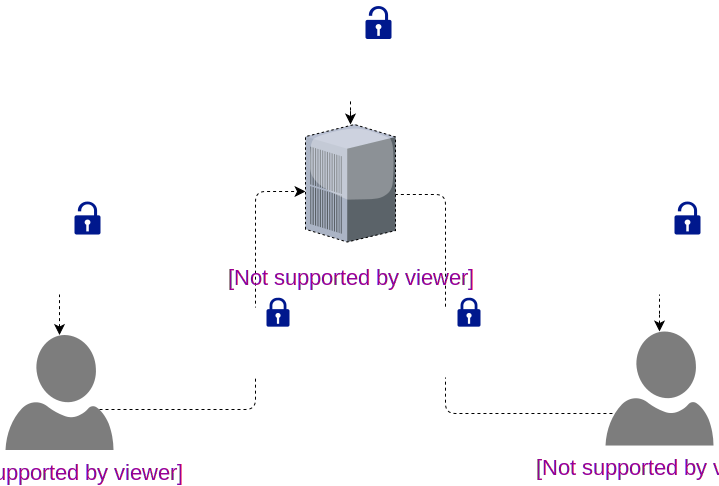
\includegraphics[width=\textwidth]{Figures/SNS}
  \decoRule
  \caption[False E2E encryption]{False end-to-end encryption used in some SNS. This allows the service to decrypt the data you send.}
  \label{fig:sns}
\end{figure}

The use of cloud services has exploded in recent times. The situation today is that if the file-attachment is too large, it will often be uploaded to a cloud-service instead and a link to said file attached. While this sort of functionality is easy to use, it makes you lose control over your data. You are giving a company access to the file that was intended only for the receiver. In reality, you are giving away ownership of the data and you no longer have control over how long it is stored, how it is stored or who can access it. You are at the mercy of the service provider. While it is doubtful that these service providers facilitate attackers and sharing of private data, one would be very naive to assume that it can not be stolen. There are countless examples of such services being successfully attacked or information being leaked on accident. A few examples are:
\begin{itemize}
	\item Celebgate/The Fappening:\\
	Attackers gained access to victims iCloud, by Apple, and gained access to large amounts of private pictures, videos and other data from celebrities \cite{CelebgateTwoMethodological}.
	\item Verizon leak:\\
	A misconfiguration in the cloud-storage of telecommunications company Verizon, exposed the personal information of up to 14 million American customers \cite{CloudLeakHow}.
	\item INSCOM leak:\\
	A large amount of critical data belonging to the United States Army Intelligence and Security Command leaked onto the public Internet \cite{osullivanBlackBoxRed}.
\end{itemize}

There are also a plethora of SNS that support file transfers. Many of these services boast of being 'end-to-end'-secure and protecting users privacy. Unfortunately, since there is no way for the users to know how each service handles their information, there is no way to know how secure their solutions really are. There is a precedent for being wary of these services though, as some have been revealed to only encrypt data between end-nodes and the server, like shown in \Cref{fig:sns}.  One example of this is Skype \cite{greenwaldMicrosoftHandedNSA2013,popaSkypeProvidedBackdoor,ItSafeTransfer}. While other services may not work the same way, the fact of the matter is that anything going through or being stored on their servers, is out of reach for you as an end user. Would it not be better if you could transfer the file directly to the intended receiver, and be in full control over where the file is?
%
\section{Contributions}
%Todo review
The intended use case for SendIt as a system, is when transferring sensitive files. For whatever reason one might have to keep data private and confidential, when one has a need to transfer such data online, SendIt will be able to provide the necessary service.

One example may be for companies transferring personnel-files between their offices. A lot of companies outsource data storage and management. As such, sending personnel-files, which then get uploaded to a cloud storage may in fact be illegal, since the company is no longer in full control of the data. This is an unnecessary risk, as direct transfer is quicker, easier and limits liability in these cases. Not only that, but it also removes the need for storing the file somewhere in transit, which removes the risk of it being stolen if an attacker gains access at a later date. We can conclude that in cases as these, SendIt is an overall improvement compared to the current alternative. The arguments for this example can be used for any transfer of sensitive or private data, and as such is applicable to a variety of scenarios. Thus, the use cases of SendIt are many, but focused around transfer confidential or private data.

Many solutions to share files already exists, with a few mentioned above. (\ref{sec:related}) The exchange and management of identities combined with peer-to-peer transfer and trust evaluation is original to SendIt. The combination of these technologies into a singular system, constitutes my original research activity. 
\paragraph{}
This thesis contributions can be summarized as follows:
%
\begin{itemize}
	%
	\item Serverless implementation of WebRTC in larger systems\\
	This thesis goes to show that serverless implementations of WebRTC can be used in larger systems. The thesis evaluates the advantages and disadvantages of such a solution in contrast to more commonly used solutions, both for WebRTC and other technologies. The advantages of not having a server broker all connections are many, and if IPv6 becomes more popular, an increase in such solutions are likely to occur due to the fact that NAT traversal will no longer be necessary. This in turn makes it easier to connect directly to endpoints. It would also allow for companies to provide services while lowering the cost of providing such services since they no longer need to provide servers to broker connections, greatly increasing profit margins. This would be very beneficial, especially for VOIP solutions, which is currently one of WebRTCs main usages.
	%
	\item Client-only development\\
	A benefit following the serverless approach, is that only a client application is necessary to use the service. No centralized program or dedicated servers are required for the service to stay operational. This reduces development time, resourced needed, lowers attack surface and results in simpler implementations. Many programs exists only locally, but being able to communicate over the internet using such programs is rare. Usually at least one connection to a centralized server or node is required for such programs to work. This is not the case for SendIt, and as such opens up a new venue for application development.
	%
	\item Propose a new system that can be expanded as needed\\
	A system offering endpoint authentication and direct P2P connections, while still being easy to use is non-existent in todays technical environment. By introducing such a system, better security becomes available to the masses. It also functions as a platform which one can modify and build on to improve current functionality, or add new ones. It is easily expandable and can be used as a platform for any kind of application over the internet. It lays the groundwork, so others can focus on the specifics of their solution, instead of worrying about connection setup or authentication of users.
	%
	\item Direct connections between users\\
	%TODO review
	As mentioned in the \Cref{sec:motivation}, one of the goals of this thesis is to go back to the idea of a decentralized internet. A direct connection, when possible, is a big step in the right direction. By utilizing P2P this is easily achievable. The problem comes down to identification, authentication and protecting the integrity of the data sent. This is rarely needed however, as P2P is not commonly used in systems that require any kind of authentication. In such systems, tokens issued by a server can be used as authentication. By creating a system using P2P and avoiding the use of a central server, problem arise. These problems can be solved by combining P2P and public key cryptography, but this again raises the issue of creating trust and trust management, since this is usually taken care of by the server. By using the web of trust model, this problem can be mitigated. This type of complete system for direct connections is new and original.
	%
	\item New perspective on e-mail attachments\\
	%Review TODO
	It is about time this functionality gets a rework and improved implementation. It has been largely unchanged since it was implemented and is desperately in need of replacement. This thesis suggests a new system that can easily be implemented in both online, as well as local e-mail clients. It can be used as either a supplementary system, or a replacement. To properly replace the current system, some updates and extended functionality would have to be added to the proposed system, but most of the work will already have been taken care of. To clarify: this thesis is only one of many ways to improve the current system. A combination of solutions will probably yield the best results. What this thesis does aim to be is one of the better, if not the best, solution for those who value usability and security.
	%
	\item Security to the people\\
	%Review TODO
	From a layman's perspective, computer security as a discipline is difficult. The computer only became mainstream in the last ~25 years, and as such, society has not yet completely adjusted to this new technology, especially the security aspect of it. While most of the workforce has adjusted and can now perform their tasks on a computer, they do not have a deep understanding of how computers work. Most users are not qualified to make judgments about how secure a solution is, or how it should be used. They rely on the IT departments to serve them easy to use applications that are customized for the intended purposes. These people occasionally need access to equally secure solutions as someone with a security background, but does not have the skills to use the same tools as the security professionals. As such, applications abstracting away all the technology and allowing for easy to use, secure systems are needed. This seems largely ignored by the security-community today, as most applications are command-line utilities, or have extremely underdeveloped GUIs. SendIt tries to remedy this by being a system that allows users to focus on the task they want to accomplish - file transfer(s) - while taking care of the security and technical challenges on behalf of the user.
	%
	\item All of the above combined\\
	All items on the above list may not be original, but combined they result in a unique approach to a problem that is largely overseen. No other system has the combined properties outlined above, which makes SendIt the first of it's kind. Hopefully, this thesis will contribute to put focus on the issues raised above and lead the way for improvements and better solutions in the future.
	%
\end{itemize}
%
%
\section{Organization}
%
The thesis is organized as follows:\\
\begin{itemize}
	\item \Cref{Chapter2} explains the technology and principles used in SendIt and gives a thorough review of the background for choosing them.\\
	\item \Cref{Chapter3} goes in depth about the design and implementation of the base system that both modes share. It reviews the implementation and basis for the functionality implemented in each mode. It will also give an overview of the extendability of the system, as well as an analysis of the security of the system.\\
	\item \Cref{Chapter4} will discuss the design and implementation chosen for the two modes mode. It will show the use cases for each mode, discuss advantages and drawbacks and indicate how to best take advantage of the given functionality of each mode.\\
	\item \Cref{Chapter5} will discuss the experiments done as part of the research. It will give an overview over the motivation for doing the experiments, the methods used and the impact and findings of the experiments.\\
	\item \Cref{Chapter6} concludes the thesis by summarizing the contributions and work done. It also discusses future work and possible improvements.
\end{itemize}
